\level{0}{Methodology and Results}
\level{1}{Scope}
Following are some questions that we consider important and need to be analysed \label{important_questions}
\begin{enumerate}
    \item What types of fMOOPs confirm to restrictions on condition number of $f$? \label{question_restriction}
    \item How to determine minimum feasible value of $\alpha$ for a given problem and subsets $X_1,X_2,X_5,X_6 \subseteq X$? \label{question_alpha_feasible_range}
    \item For the fMOOPs which confirm such condition number restrictions how does the condition number behave over the domain $X_5,X_6$? \label{question_behaviour_of_cond_over_x5x6}
    \item Based on the behaviour of the condition number what types of methods do we expect to work well? \label{question_what_methods_we_expect_to_work}
    \item What all computation methods/algorithms are available for condition number w.r.t. specific fMOOP? \label{question_computation_methods}
    \item How the transformed problems with bounds on condition number behave and how close are their solutions to the original problems solutions? \label{question_transformed_problems_behaviour}
\end{enumerate}
In this analysis and results we will consider following 2 main problems derived from the problems \ref{problem_linear_factor_model} and \ref{problem_defense_adv_nn_attack}, both of which are defined in the Applications and Motivation section.


\level{1}{Theoretical Results}
\textbf{Condition number over composition of function}: Say we have a function $f=g(h(x)) = g \circ h(x)$ where $f:X\to Y$, $h:X\to Z$, and $g:Z\to Y$ then we can write
\begin{equation}
    cond_{abs}(f,x) = \underset{\epsilon \to 0}{lim}\underset{||\delta x||\le \epsilon}{sup} \frac{||\delta f(x)||}{||\delta x||} = \underset{\epsilon \to 0}{lim}\underset{||\delta x||\le \epsilon}{sup} \frac{||\delta g(h(x))||}{||\delta x||}
\end{equation}
$\implies$
\begin{equation}
    cond_{abs}(f,x) = \underset{\epsilon \to 0}{lim}\underset{||\delta x||\le \epsilon}{sup} \frac{||\delta g(h(x))||}{||\delta h(x)||}\frac{||\delta h(x)||}{||\delta x||}
\end{equation}
under the assumption that $\forall \epsilon \ge 0$ and $||\delta x||
\le \epsilon$ $\exists\hspace{1mm} \delta \ge 0$ such that $||\delta h(x)|| \le \delta$ $\forall x$ and $\underset{\epsilon \to 0}{lim}\hspace{1mm} \delta = 0$. Then we can write
\begin{equation}
    cond_{abs}(f,x) = \underset{\delta \to 0}{lim}\underset{||\delta h(x)||\le \delta}{sup} \frac{||\delta g(h(x))||}{||\delta h(x)||} \underset{\epsilon \to 0}{lim}\underset{||\delta x||\le \epsilon}{sup} \frac{||\delta h(x)||}{||\delta x||}
\end{equation}
let $h(x) = z \implies \delta h(x) = \delta z $, and since $z$ is a function of $x$, $\delta z$ is not independent of $\delta x$ hence we can write
\begin{equation}
    cond_{abs}(f,x) \le \underset{\delta \to 0}{lim}\underset{||\delta z||\le \delta}{sup} \frac{||\delta g(z)||}{||\delta z||} \underset{\epsilon \to 0}{lim}\underset{||\delta x||\le \epsilon}{sup} \frac{||\delta h(x)||}{||\delta x||}
\end{equation}
$\implies$
\begin{equation} \label{cond_fun_comp_bound}
    cond_{abs}(f,x) \le cond_{abs}(g,h(x))\times cond_{abs}(h,x)
\end{equation}
the above \ref{cond_fun_comp_bound} bound can be used to simplify the fMOOP with constraints on condition number for complex functions which are composition of simpler function whose condition number can be bound analytically, for eg. Neural Networks come under such functions.
\newline\newline \textbf{Relation between absolute and relative condition number}: given a function $f:X\to Y$ its absolute and relative condition number are given by
\begin{equation}
    cond_{abs}(f,x) = \underset{\epsilon \to 0}{lim}\underset{||\delta x||\le \epsilon}{sup} \frac{||\delta f(x)||}{||\delta x||}
\end{equation}
\begin{equation}
    cond_{rel}(f,x) = \underset{\epsilon \to 0}{lim}\underset{||\delta x||\le \epsilon}{sup} \frac{||\delta f(x)||/||f(x)||}{||\delta x||/||x||}
\end{equation}
we can write
\begin{equation}
    cond_{rel}(f,x) = \underset{\epsilon \to 0}{lim}\underset{||\delta x||\le \epsilon}{sup} \frac{||\delta f(x)||}{||\delta x||}\frac{||x||}{||f(x)||}
\end{equation}
$\implies$
\begin{equation} \label{cond_abs_rel_relation}
    cond_{rel}(f,x) = cond_{abs}(f,x)\frac{||x||}{||f(x)||}
\end{equation}
\newline\newline \textbf{$L_2$ regularization and absolute condition number}: Consider the problem of fitting data with $n$ data points $(X_i,Y_i), i \in [n]$, each column being 1 data point $(X,Y) \in (\mathbb{R}^{d\times n},\mathbb{R}^{1\times n})$ using a function $f:\mathbb{R}^{d\times 1}\to \mathbb{R}^{1\times 1}$, for case of simplicity assume $f$ is linear transform i.e. $f(X) = AX \approx Y$ where $A \in \mathbb{R}^{1\times d}$.
\newline Consider the $L_2$ regularization formulations of this problem as follows
\begin{equation} \label{l2_reg_prob_obj}
    \underset{A \in \mathbb{R}^{1\times d}}{min}\hspace{1mm} \frac{1}{n}\mathlarger{\sum}_{i\in [n]} ||AX_i-Y_i||_2 + \lambda ||A||^{2}_{2}
\end{equation}
Now, consider the same problem under fMOOP for minimizing the $||\cdot||_{F}$ frobenius norm of the transform $A$ over the aggregation scheme of mean and $X_3 = \mathbb{R}^{d\times 1}$
\begin{equation} \label{fmoop_l2_rel_obj_1}
    \underset{A \in \mathbb{R}^{1\times d}}{min}\hspace{1mm} \frac{1}{n}\mathlarger{\sum}_{i\in [n]} ||AX_i-Y_i||_2
\end{equation}
\begin{equation} \label{fmoop_l2_rel_obj_2}
    \underset{A \in \mathbb{R}^{1\times d}}{min}\hspace{1mm} \underset{x \in X_3}{max}\hspace{1mm} cond_{abs}(f,x)
\end{equation}
by definition 
\begin{equation}
    cond_{abs}(f,x) = \underset{\epsilon \to 0}{lim}\underset{||\delta x||_F\le \epsilon}{sup} \frac{||A\delta x||_F}{||\delta x||_F}
\end{equation}
note that $||A\delta x||_F = \sqrt{(\sum_{i\in [d]} A_i\delta x_i)^2}$ and by Cauchy–Schwarz inequality we can write $(\sum_{i\in [d]} A_i\delta x_i)^2 \le (\sum_{i\in [d]} A^2_i)(\sum_{i\in [d]} x^2_i) =||A||^2_F||\delta x||^2_F $, which implies 
\begin{equation} \label{cond_forb_ub_1d}
    cond_{abs}(f,x) = \underset{\epsilon \to 0}{lim}\underset{||\delta x||_F\le \epsilon}{sup} \frac{||A\delta x||_F}{||\delta x||_F} \le \frac{||A||_F||\delta x||_F}{||\delta x||_F} = ||A||_F
\end{equation}
note that for this case $||\cdot||_F$ is equivalent to $||\cdot||_2$, and the above upper bound implies that the problem \ref{fmoop_l2_rel_obj_2} when minimized for the worst case using the upper bound \ref{cond_forb_ub_1d} we get the fMOOP as follows
\begin{equation} \label{fmoop_l2_rel_obj_new}
    \underset{A \in \mathbb{R}^{1\times d}}{min}\hspace{1mm} (||A||_2, \frac{1}{n}\mathlarger{\sum}_{i\in [n]} ||AX_i-Y_i||_2)
\end{equation}
which when scalarized with squaring the norm restriction gives us the standard $L_2$ regularization.

\level{1}{Experimental Results}
\level{2}{Problem: Linear Factor Model} \label{results_problem_1}
This is the same problem as defined in the section \ref{problem_linear_factor_model}.
\newline A data of returns for $n$ time series $R^{n\times 1}_t \in \mathbb{R}^{n\times 1}$, for $t\in [T]$ and denote $R^{n\times d}_{t\times d} = [R^{n\times 1}_{t-1},R^{n\times 1}_{t-2},...,R^{n\times 1}_{t-d}] \in \mathbb{R}^{n\times d}$ is given.
\newline \newline We need to design $A^{d\times k} \in  \mathbb{R}^{d\times k}$ and $\beta^{k\times 1} \in \mathbb{R}^{k\times 1}$, such that $F^{n\times k}_t = R^{n\times d}_{t\times d}\times A^{d\times k}$ and $P^{n \times 1}_{t} = F^{n\times k}_t \times \beta^{k \times 1}$ and $P^{n \times 1}_{t} \approx R^{n \times 1}_{t}$. And the performance  which is measured by \textit{Average} aggregation scheme over the loss function $\mathcal{L}(y,\hat{y}) = ||y-\hat{y}||_2$ which we need to minimize and another \textit{Average} aggregation scheme over the return function $\mathcal{R}(y,\hat{y}) = \frac{\langle y,\hat{y}\rangle}{||y||_2||\hat{y}||_2}$ defined over the testing period of $t \in [T,T+S]= \{T,T+1,...,T+S-1\}$ which we need to maximize.

\begin{equation} \label{results_problem_lfm_diagram}
\begin{tikzcd}
R^{n\times d}_{t \times d} \arrow[rr, "\times A^{d\times k}" description] \arrow[r, no head]& {}& F^{n\times k}_{t} \arrow[d, "\times \beta^{k\times 1}" description] \\
R^{n\times 1}_t \arrow[rr, "\mathcal{L}" description, Rightarrow, no head] \arrow[rd, dashed] && P^{n \times 1}_{t} \arrow[ld, dashed]\\
& \mathcal{R} &
\end{tikzcd}
\end{equation}
\newline
And the orthonormal condition
\begin{equation} \label{results_problem_orthonormal_eq}
 A^{d\times k}(A^{d\times k})^{\top} = I^{d\times d}
\end{equation}
From the \ref{results_problem_orthonormal_eq} we can infer that $(A^{d\times k})^\top$ belongs to the set of right inverses of $A^{d\times k}$. 
\newline With the two objectives as:
\begin{equation} \label{problem_lfm_loss}
\underset{\beta^{k \times 1}\in \mathbb{R}^{k\times 1}, A^{d\times k} \in \mathbb{R}^{d\times k}}{min}\hspace{1mm} \mathcal{L}_{\beta^{k \times 1}, A^{d\times k}}
\end{equation}
Where $\mathcal{L}_{\beta^{k \times 1}, A^{d\times k}}$ is defined as follows
\begin{equation} \label{problem_lfm_loss_exprr}
\mathcal{L}_{\beta^{k \times 1}, A^{d\times k}} = \frac{1}{T-d+1} \mathlarger{\mathlarger{\sum}}_{\forall t\in [d,T]} \hspace{1mm} ||R^{n\times 1}_t-R^{n\times d}_{t\times d}\times A^{d\times k} \times \beta^{k \times 1}||_2^2
\end{equation}
and 
\begin{equation} \label{problem_lfm_reward}
\underset{\beta^{k \times 1}\in \mathbb{R}^{k\times 1}, A^{d\times k} \in \mathbb{R}^{d\times k}}{max}\hspace{1mm} \mathcal{R}_{\beta^{k \times 1}, A^{d\times k}}
\end{equation}
Where $\mathcal{R}_{\beta^{k \times 1}, A^{d\times k}}$ is defined as follows
\begin{equation} \label{problem_lfm_reward_exprr}
\mathcal{R}_{\beta^{k \times 1}, A^{d\times k}} = \frac{1}{S} \mathlarger{\mathlarger{\sum}}_{\forall t\in [T,T+S]} \hspace{1mm} \frac{\langle R^{n\times 1}_t,R^{n\times d}_{t\times d}\times A^{d\times k} \times \beta^{k \times 1}\rangle}{||R^{n\times 1}_t||_2||R^{n\times d}_{t\times d}\times A^{d\times k} \times \beta^{k \times 1}||_2}
\end{equation}
\level{3}{Data}
We will be using the data provided by \textit{Qube Research and Technologies (QRT)} on the \textit{Challenge Data} site, under the challenge: \textit{Learning factors for stock market returns prediction} \cite{qrt_challenge}.\newline The data contains (cleaned) daily returns of 50 stocks over a time period of 754 days (three years). And in the original problem they have asked for solutions with $d=250$ and $k=10$.
% \begin{figure}[htbp]
%     \centering
%     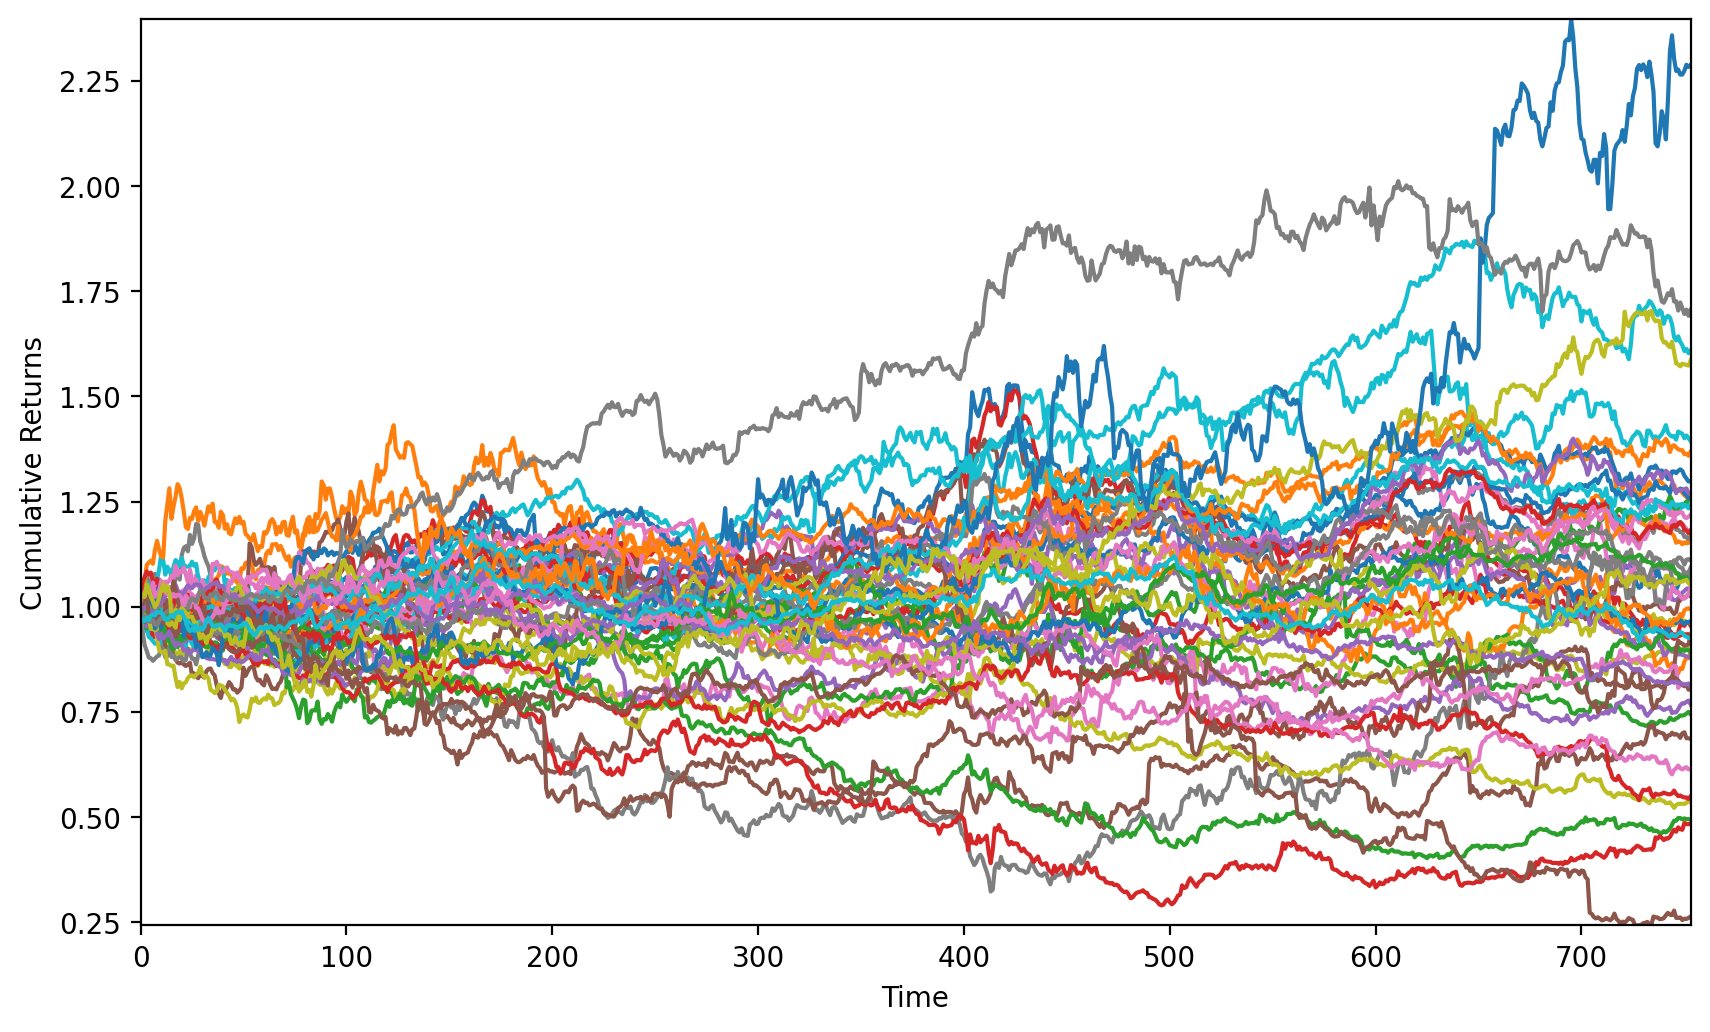
\includegraphics[width=0.8\textwidth]{images/cumulative_returns_qrt_timeseries_data.png}
%     \caption{Cumulative Returns for Daily Returns Time Series}
%     \label{fig:cumulative_returns}
% \end{figure}
% \begin{figure}[htbp]
%   \centering
%   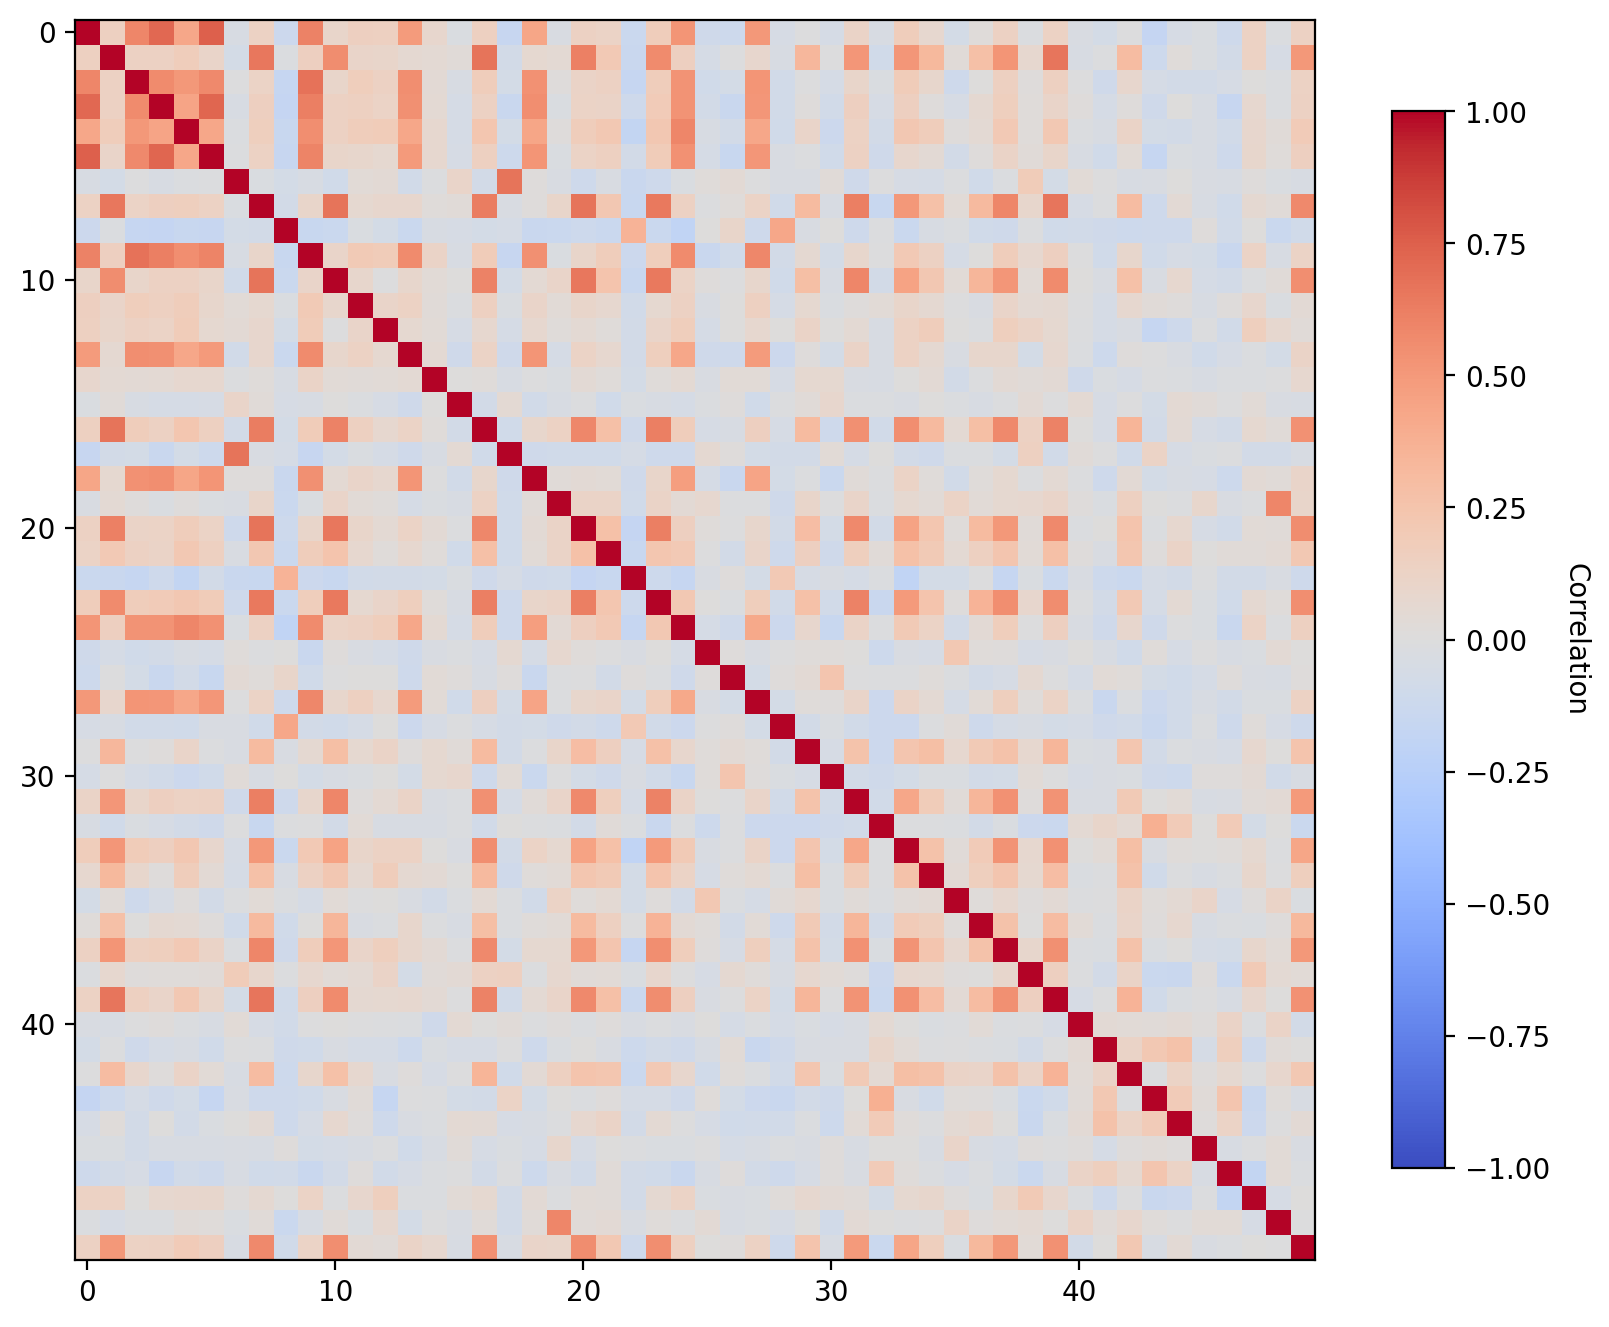
\includegraphics[width=0.9\textwidth]{images/correlation_matrix_50by50_timeseries_qtr_data.png}
%   \caption{Correlation Matrix for returns of 50 time series}
%   \label{fig:corr_matrix_ts_qrt_data}
% \end{figure}

\begin{figure}[H]
    \centering
    \begin{minipage}[t]{0.5789\textwidth}
        \centering
        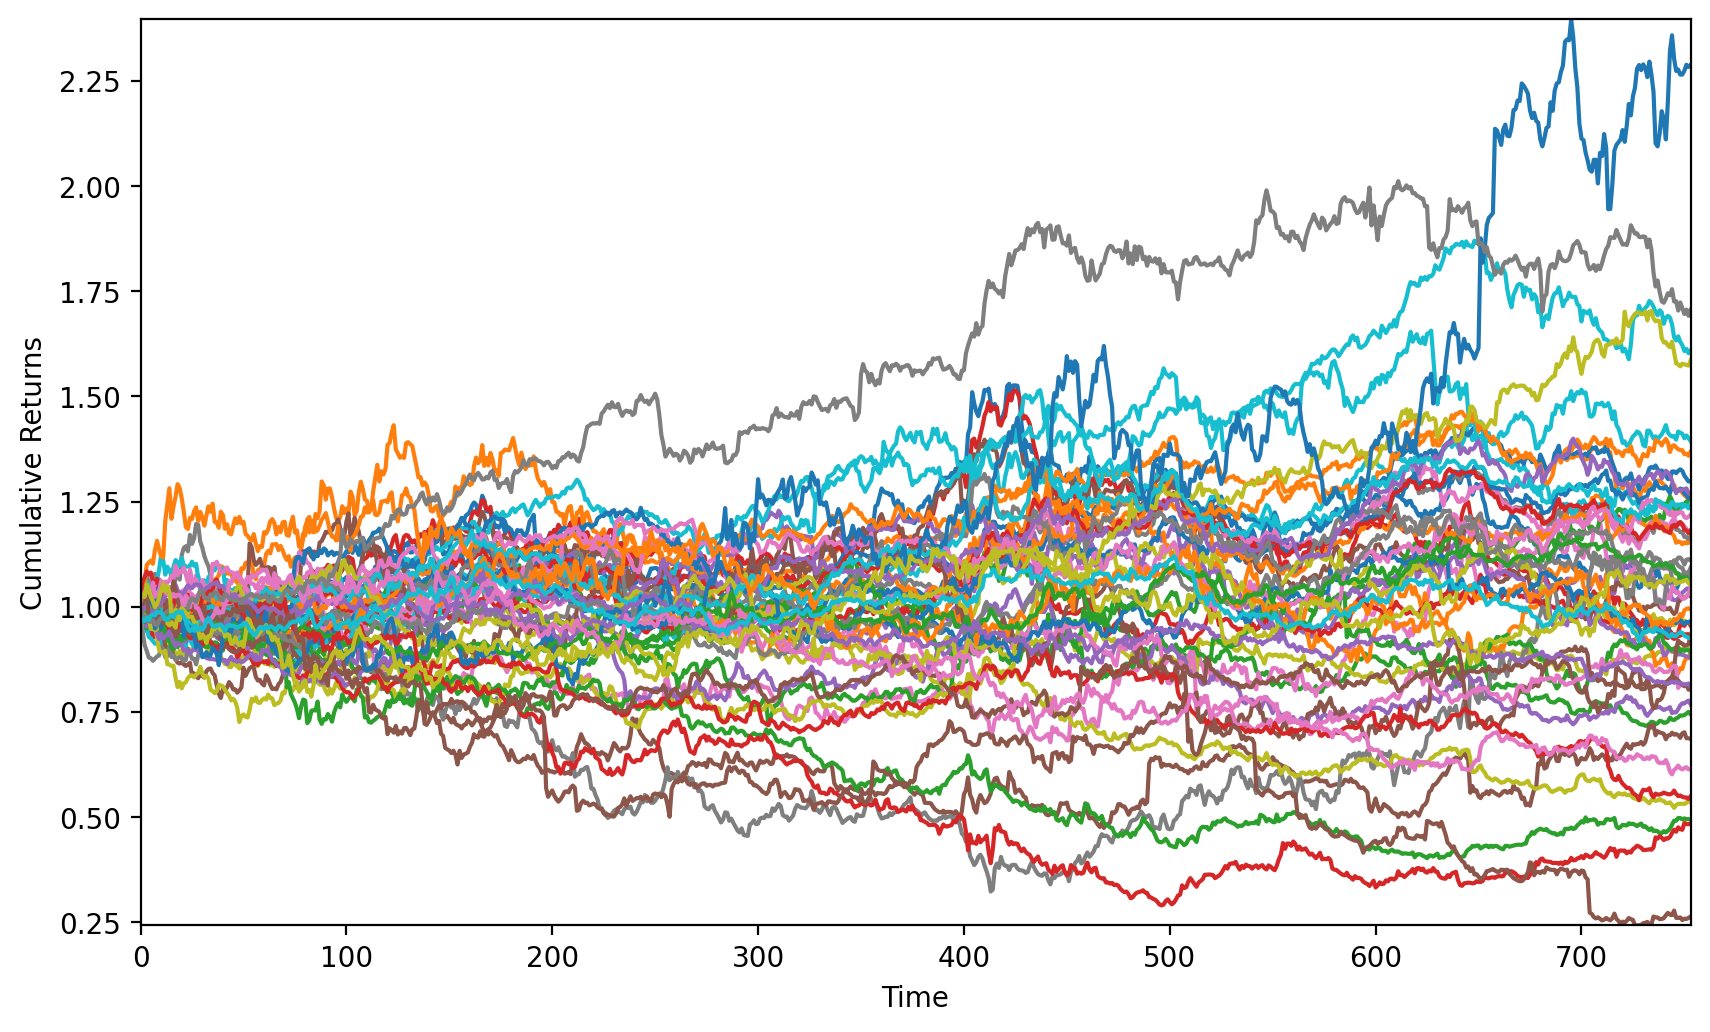
\includegraphics[width=\textwidth]{images/cumulative_returns_qrt_timeseries_data.png}
        \captionsetup{font=tiny}
        \caption{Cumulative Returns for Daily Returns Time Series}
        \label{fig:cumulative_returns}
    \end{minipage}%
    \begin{minipage}[t]{0.4211\textwidth}
        \centering
        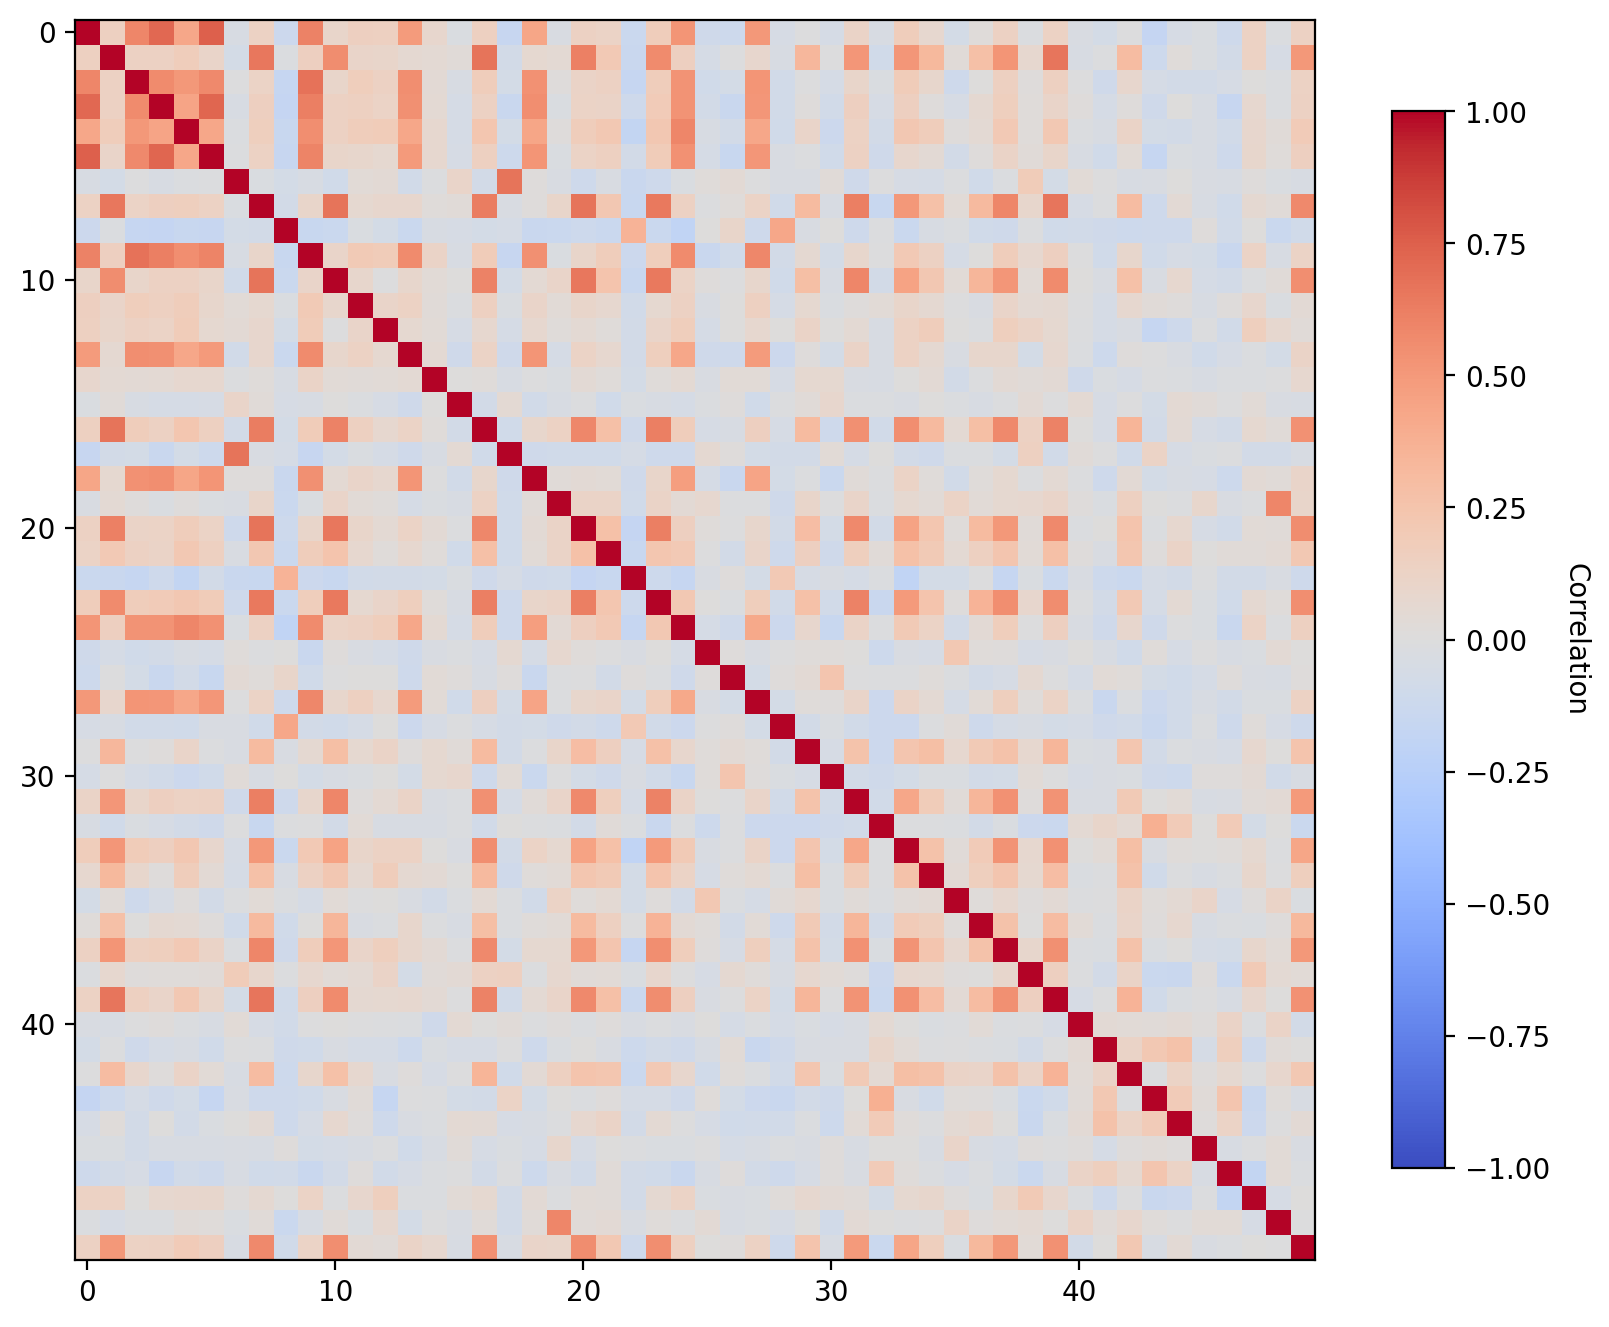
\includegraphics[width=\textwidth]{images/correlation_matrix_50by50_timeseries_qtr_data.png}
        \captionsetup{font=tiny}
        \caption{Correlation Matrix of Daily Returns}
        \label{fig:corr_matrix_ts_qrt_data}
    \end{minipage}
\end{figure}
\begin{figure}[H]
  \centering
  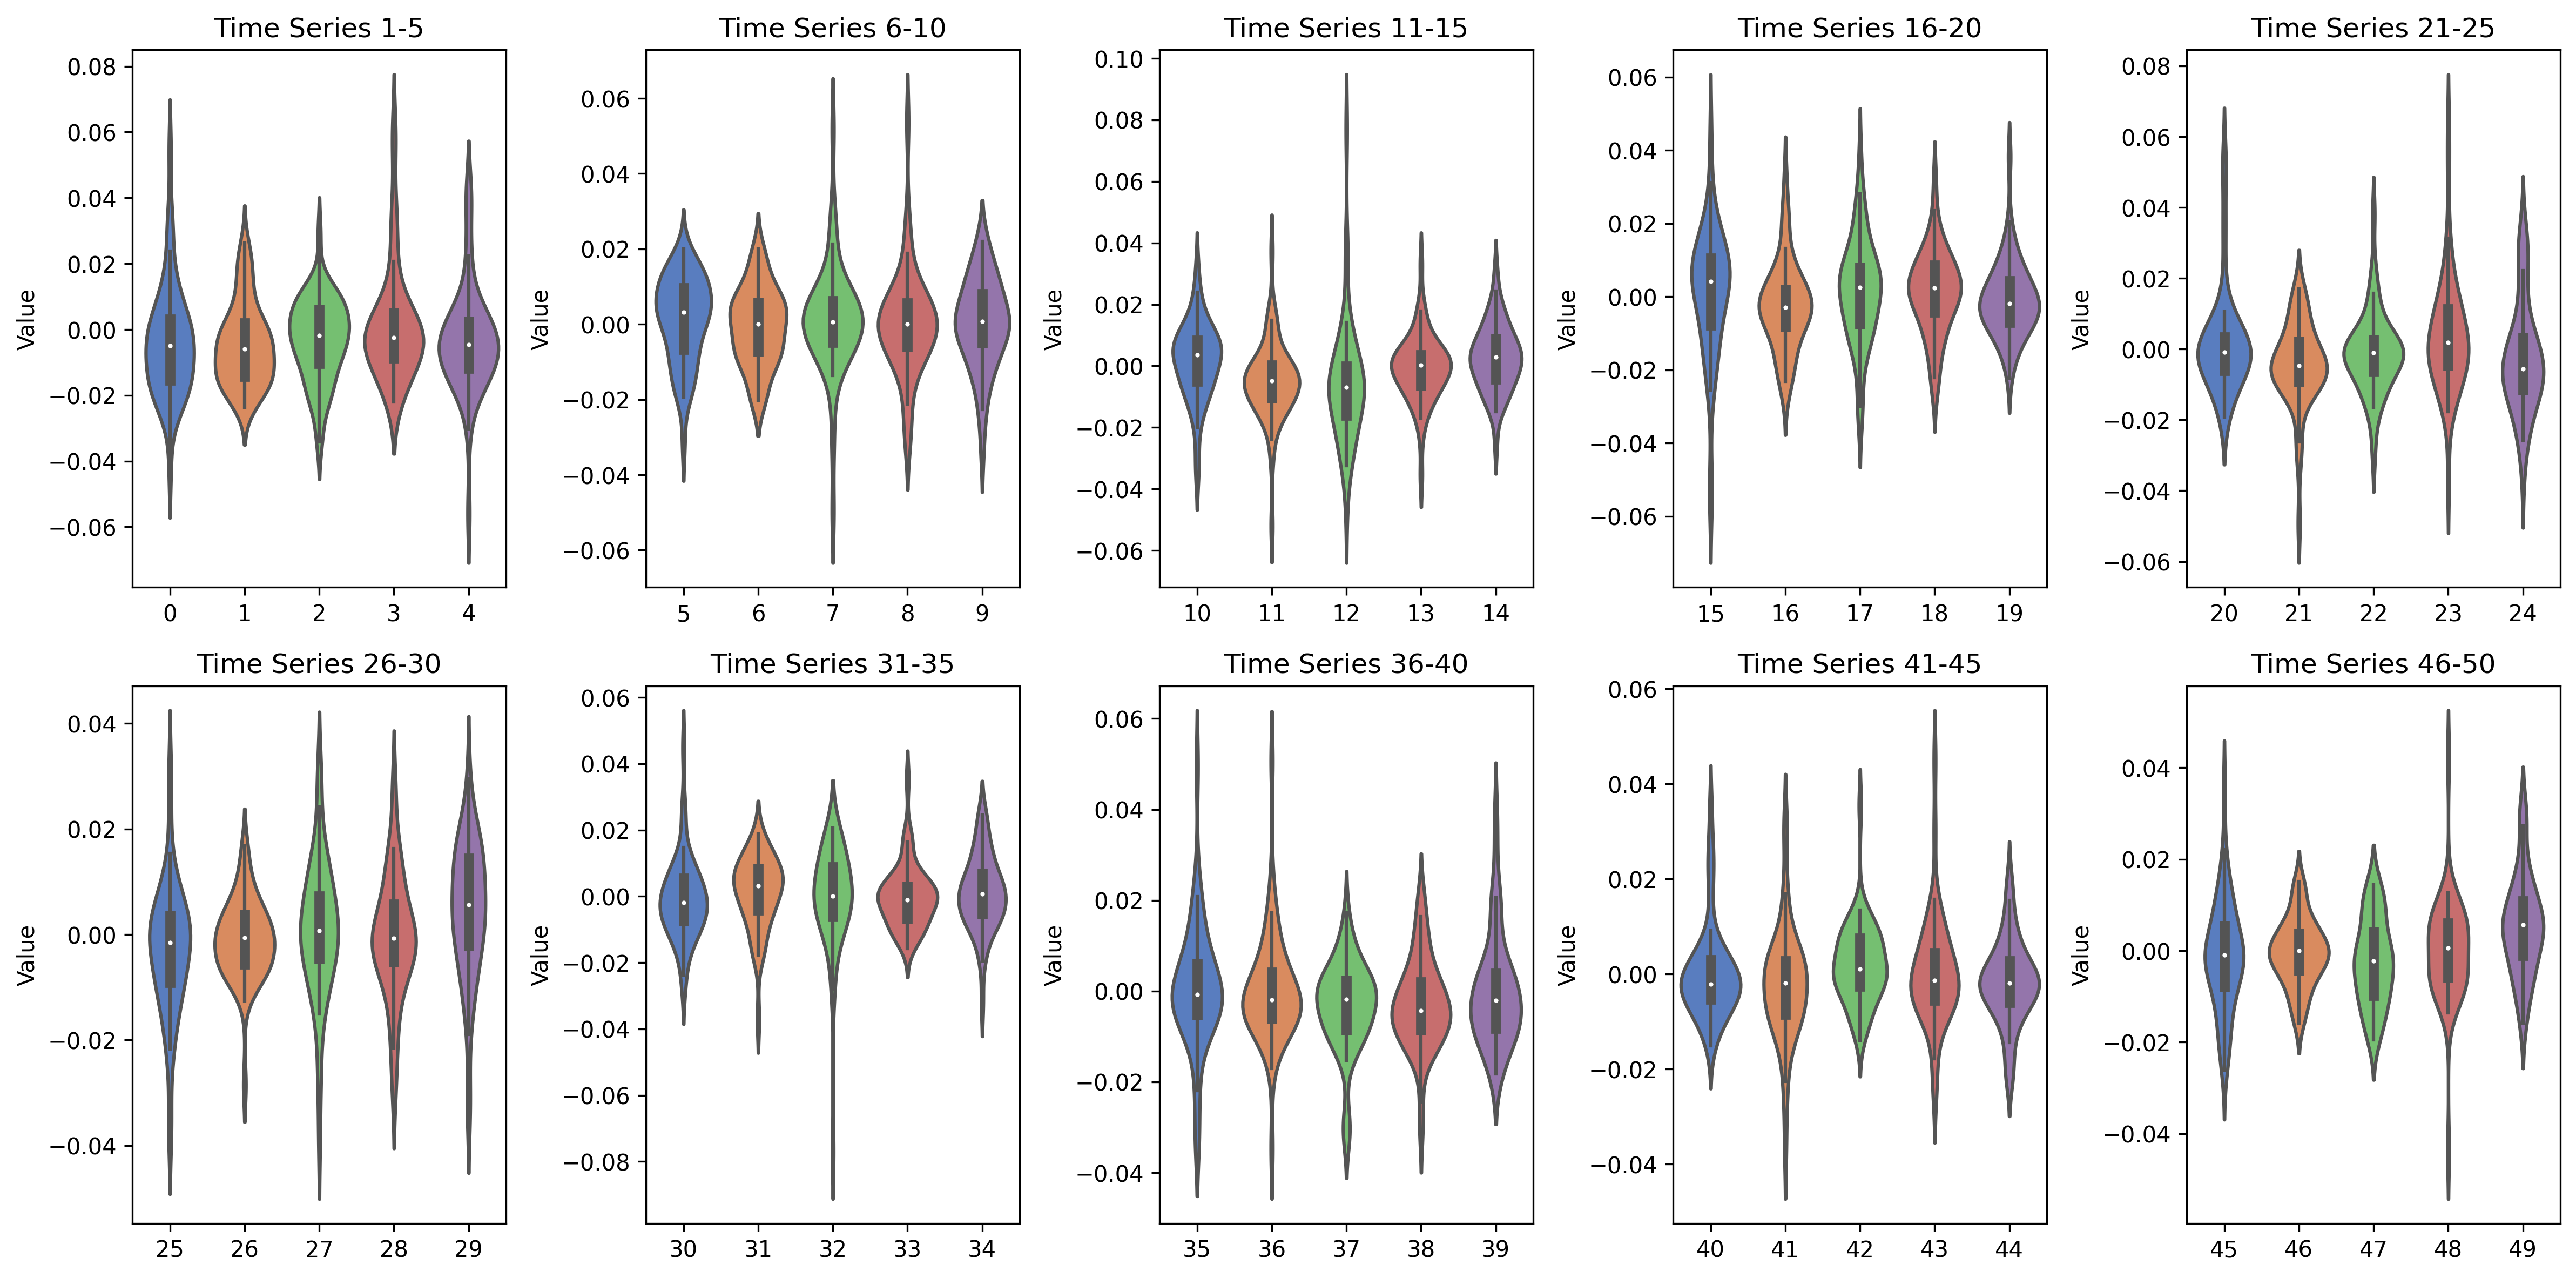
\includegraphics[width=\textwidth]{images/violin_plots_50_timeseries.png}
  \caption{Violin Plots for 50 Time Series}
  \label{fig:violin_plots}
\end{figure}

\level{3}{Approaches}
\level{4}{Baseline Method} The following method is based on randomized sampling method, which involves generating the matrix $M$ randomly and applying random data and fitting them to the training data set using linear regression. This process is repeated multiple times, and the best result is selected from the attempts.
Following is the pseudocode for the method:
\begin{algorithm}[H]
\caption{$\mathcal{A}_{0}$ : Baseline Method}\label{lfm_baseline_method}
\begin{algorithmic}[1]
\Require{$N_{iter}$}
\Ensure{$\beta_{optimal}, A_{optimal}, \mathcal{R}_{optimal} \gets \emptyset, \emptyset, -\infty $}
\For{$i \gets 1 ... N_{iter}$}
    \State $M_i \gets sample\_random\_matrix()$
    \State $A_i \gets gram\_schmidt\_algorithm(M_i)$\Comment{orthonormalize $M_i$ to $A_i$}
    \State Compute $\{F^{n\times k}_{t, i}\}$ for $A_i$ over $t\in [d,T]$
    \State $\beta_i \gets regression(\{R^{n\times 1}_{t}\},\{F^{n\times k}_{t, i}\}, t\in [d,T])$
    \If{$\mathcal{R}_{\beta_i, A_i} > \mathcal{R}_{optimal}$}  \Comment{update the optimal if better solution found}
        \State $\beta_{optimal}, A_{optimal}, \mathcal{R}_{optimal} \gets \beta_{i}, A_{i}, \mathcal{R}_{\beta_i, A_i} $
    \EndIf 
\EndFor
\end{algorithmic}
\end{algorithm} In an alternate implementation of this algorithms we can even do grid search over the entries of $A$, but because of the high number of possibilities we restrict this method over randomized search. 
\level{4}{Gradient Based Methods}
To compute the partial derivatives of the loss function $\mathcal{L}_{\beta^{k \times 1}, A^{d\times k}}$ with respect to $A^{d\times k}$ and $\beta^{k \times 1}$, we will use the chain rule and the derivative of the matrix multiplication.\newline \newline First, let's compute the derivative of $\mathcal{L}_{\beta^{k \times 1}, A^{d\times k}}$ with respect to $\beta^{k \times 1}$. Lets Define $\Delta_t = R^{n\times 1}_t-R^{n\times d}_{t\times d}\times A^{d\times k} \times \beta^{k \times 1}$
\begin{equation}
    \frac{\partial \mathcal{L}_{\beta^{k \times 1}, A^{d\times k}}}{\partial \beta^{k \times 1}} = \frac{1}{T-d+1} \sum_{\forall t\in [d,T]} \frac{\partial}{\partial \beta^{k \times 1}} ||\Delta_t||_2^2 
\end{equation}
\newline Now, let's compute the derivative of $||\Delta_t||_2^2$ with respect to $\beta^{k\times 1}$:

\begin{equation}
    \frac{\partial}{\partial \beta^{k \times 1}} ||\Delta_t||_2^2 =  \frac{\partial}{\partial \beta^{k \times 1}} \Delta_t^\top \Delta_t = 2F_t^\top (F_t \beta - R_t)
\end{equation}
\newline Which gives
\begin{equation}
    \frac{\partial \mathcal{L}_{\beta^{k \times 1}, A^{d\times k}}}{\partial \beta^{k \times 1}} = \frac{2}{T-d+1} \sum_{\forall t\in [d,T]} F_t^\top (F_t \beta - R_t)
\end{equation}
\newline Similarly consider 
\begin{equation}
    \frac{\partial \mathcal{L}_{\beta^{k \times 1}, A^{d\times k}}}{\partial A^{d \times k}} = \frac{1}{T-d+1} \sum_{\forall t\in [d,T]} \frac{\partial}{\partial A^{d \times k}} ||\Delta_t||_2^2 
\end{equation}
We will use the following identities when $a$, $b$ and $C$ are not functions of $X$.
\begin{equation} \label{matrix_calc:id1}
\frac{\partial (\mathbf{a}^\top \mathbf{X} \mathbf{b})}{\partial \mathbf{X}} = \mathbf{a} \mathbf{b}^\top
\end{equation}
\begin{equation}\label{matrix_calc:id2}
\frac{\partial (\mathbf{a}^\top \mathbf{X}^\top \mathbf{b})}{\partial \mathbf{X}} = \mathbf{b} \mathbf{a}^\top
\end{equation}
\begin{equation}\label{matrix_calc:id3}
\frac{\partial (\mathbf{X} \mathbf{a})^\top \mathbf{C} (\mathbf{X} \mathbf{b})}{\partial \mathbf{X}} = \mathbf{C} \mathbf{X} \mathbf{b} \mathbf{a}^\top + \mathbf{C}^\top \mathbf{X} \mathbf{a} \mathbf{b}^\top
\end{equation}
\newline for the equations below we are dropping the dimensions
\begin{equation}
    ||\Delta_t||_2^2 = \Delta_t^\top \Delta_t = (R_t-R_{t\times d} A  \beta)^\top (R_t-R_{t\times d} A \beta) = R_t^\top R_t
\end{equation}
\begin{equation}
    ||\Delta_t||_2^2 = R_t^\top R_t - R_t^\top R_{t\times d} A \beta - \beta^\top A^\top  R_{t\times d}^\top R_t+ \beta^\top A^\top  R_{t\times d}^\top R_{t\times d} A \beta
\end{equation}
\newline Now using the identities \ref{matrix_calc:id1}, \ref{matrix_calc:id2}, \ref{matrix_calc:id3} we get 
\begin{equation}
    \frac{\partial}{\partial A} ||\Delta_t||_2^2 = 2(R_{t\times d}^\top R_{t\times d} A \beta \beta^\top - R_{t\times d}^\top R_t \beta^\top)
\end{equation}
\newline Which gives
\begin{equation}
    \frac{\partial \mathcal{L}_{\beta, A}}{\partial A} = \frac{2}{T-d+1} \sum_{\forall t\in [d,T]} R_{t\times d}^\top R_{t\times d} A \beta \beta^\top - R_{t\times d}^\top R_t \beta^\top
\end{equation}
\newline For vector-valued scalar functions $v(\mathbf{x})$ and $u(\mathbf{x})$ with respect to $\mathbf{x}$, and where $A$ is not a function of $x$.

\begin{equation}\label{eq:partial-derivative-vector-function}
\frac{\partial}{\partial \mathbf{x}} \left( v(\mathbf{x}) u(\mathbf{x}) \right) =  v \frac{\partial u}{\partial \mathbf{x}} + \frac{\partial v}{\partial \mathbf{x}} u
\end{equation}
\begin{equation}\label{eq:partial-derivative-matrix-function}
\frac{\partial}{\partial \mathbf{x}} (\mathbf{x}^{\top} \mathbf{A} \mathbf{x}) = (\mathbf{A} + \mathbf{A}^{\top}) \mathbf{x}
\end{equation}
\begin{equation}
\frac{\partial (\mathbf{Ax})}{\partial \mathbf{x}} = \mathbf{A}^\top \label{eq:partial_Ax_wrt_x}
\end{equation}
\newline define $\rho_t = \frac{\langle R_t,R_{t\times d} A  \beta\rangle}{||R_t||_2||R_{t\times d} A \beta||_2} = \frac{ R_t^\top R_{t\times d} A  \beta}{||R_t||_2||R_{t\times d} A \beta||_2} = \frac{ R_t^\top F_t \beta}{||R_t||_2||F_{t} \beta||_2}$ and $\hat{R}_t=\frac{R_t}{||R_t||_2}$, now using \ref{eq:partial-derivative-matrix-function}, \ref{eq:partial-derivative-vector-function}, \ref{eq:partial_Ax_wrt_x}, \ref{matrix_calc:id1} and \ref{matrix_calc:id3} we get
\begin{equation} \label{eq:derivative-rho_t_beta}
    \frac{\partial \rho_t}{\partial \beta} =  \frac{1}{||F_t\beta||_2}F_t^\top \hat{R}_t - \frac{2F_t^\top F_t \beta}{2||F_t\beta||_2^3}\hat{R}_t^\top F_t \beta
\end{equation}
\begin{equation} \label{eq:derivative-rho_t_A}
    \frac{\partial \rho_t}{\partial A} =  \frac{1}{||F_t\beta||_2} R_{t\times d}^\top \hat{R}_t \beta^\top - \frac{2R_{t\times d}^\top R_{t\times d} A \beta \beta^\top }{2||F_t\beta||_2^3}\hat{R}_t^\top F_t \beta
\end{equation}
\newline From that we can get
\begin{equation}
    \frac{\partial \mathcal{R}_{\beta, A}}{\partial A} = \frac{1}{S} \mathlarger{\mathlarger{\sum}}_{\forall t\in [T,T+S]} \hspace{1mm} \frac{\partial \rho_t}{\partial A} 
\end{equation}
\begin{equation}
    \frac{\partial \mathcal{R}_{\beta, A}}{\partial \beta} = \frac{1}{S} \mathlarger{\mathlarger{\sum}}_{\forall t\in [T,T+S]} \hspace{1mm} \frac{\partial \rho_t}{\partial \beta} 
\end{equation}
\newline Also we can get derivative w.r.t. $A$ for the frobenius norm of $AA^\top-I$
\begin{equation} \label{eq:derivative_forb_norm_ofAAtmI}
    \frac{\partial ||AA^\top-I||_F}{\partial A} = -4\cdot (I-A\cdot A^\top )\cdot A
\end{equation}
\textbf{Observation}\newline 
Consider the set of matrices $\mathcal{O}_d^k = \{ A | AA^\top = I_d, A \in \mathbb{R}^{d\times k} \}$, observe that $\mathcal{O}_k^k$ is set of all orthonormal square matrix of size $k\times k$ and for a $Q\in \mathcal{O}_k^k$ we have $QQ^\top = I$, which implies $Q^{-1}= Q^\top$ and hence $QQ^\top = Q^\top Q = I$. Using the aforementioned fact we observe that $AQ\in \mathcal{O}_d^k$ as
\begin{equation} \label{observation:ortho-closure_odk}
    (AQ)(AQ)^\top = AQQ^\top A^\top = AA^\top 
\end{equation}
Now consider and iterative scheme for finding $A, \beta$ which generates $\{A_i, \beta_i\}_{i=0}^{N_{iter}}$ with updates at $i$'th iteration denoted as $\{\Delta A_i, \Delta \beta_i\}$
\begin{equation}
\begin{aligned}
    A_{i+1} = A_i + \Delta A_i \\
    \beta_{i+1} = \beta_i + \Delta \beta_i
\end{aligned}
\end{equation}
But since in our problem we have added restriction on $A \in \mathcal{O}_d^k$, which we can solve by one of the following 2 approaches 
\newline \newline \textbf{General approaches to satisfy orthonormality condition}
\begin{enumerate}
    \item Design the iteration scheme such that $A_i \in \mathcal{O}_d^k, \forall i \in \{0,1,2,...,N_{iter}\}$
    \item Relax the Condition on $A \in \mathcal{O}_d^k$ to $A \in \mathbb{R}^{d\times k}$ and solve using an iterative scheme;  then project $A_{N_{iter}}$ to $\mathcal{O}_d^k$ i.e. solve the problem $\underset{\beta \in \mathbb{R}^{k \times 1}, A \in \mathcal{O}_d^k}{min} \hspace{2mm} ||A_{N_{iter}}-A||$ subject to $\mathcal{R}_{\beta, A} \ge \mathcal{R}_{\beta_{N_{iter}}, A_{N_{iter}}}$ $\mathcal{L}_{\beta, A} \le \mathcal{L}_{\beta_{N_{iter}}, A_{N_{iter}}}$
\end{enumerate}
First we will use the observation \ref{observation:ortho-closure_odk} to design an iterative scheme such that $A_i \in \mathcal{O}_d^k, \forall i \in \{0,1,2,...,N_{iter}\}$
\newline Lets say via some iterative method we get $\Delta A_i$ update for $A_i$ but since $A_{i+1} = A_i + \Delta A_i$ need not belong to $\mathcal{O}_d^k$ we need some way to project $\Delta A_i$ in a space such that $A_{i+1} \in \mathcal{O}_d^k$
\newline We define $\mathcal{O}_d^k$
\begin{equation}
    \delta \mathcal{O}_d^k = \{ \delta | \delta = A - B, A, B \in \mathcal{O}_d^k \}
\end{equation}
which implies, we require to project $\Delta A_i$ in $\delta \mathcal{O}_d^k $ or to say $\Delta A_i \to proj_{\delta \mathcal{O}_d^k}(\Delta A_i)$
\newline \newline \textbf{Properties of $\mathcal{O}_d^k $}
\begin{enumerate}
    \item $A \in \mathcal{O}_d^k \implies -A \in \mathcal{O}_d^k$ \label{odk_prop:prop1}
    \item $A \in \mathcal{O}_d^k$ and $Q\in \mathcal{O}_k^k$ we have $A Q \in \mathcal{O}_d^k$ as in \ref{observation:ortho-closure_odk}
\end{enumerate}
\textbf{Properties of $\delta \mathcal{O}_d^k $}
\begin{enumerate}
    \item $\bar{\textbf{0}} \in \delta \mathcal{O}_d^k$
    \item $A, B \in \mathcal{O}_d^k$ we have $A-B, A+B \in \delta \mathcal{O}_d^k$ as by property \ref{odk_prop:prop1} of $\mathcal{O}_d^k$
    \item $\delta \in \delta \mathcal{O}_d^k$ and $Q\in \mathcal{O}_k^k$ we have $\delta Q \in \delta \mathcal{O}_d^k$ by \ref{observation:ortho-closure_odk}
\end{enumerate}
So if we could get an associated $Q_i \in \mathcal{O}_k^k$ with $\Delta A_i$ such that we can replace $A_{i+1} = A_i+proj_{\delta \mathcal{O}_d^k}(\Delta A_i)$ with $A_{i+1} = A_iQ_i$  
\newline As per the property of $\delta \mathcal{O}_d^k$ for $A, B \in \mathcal{O}_d^k$ we have $A-B, A+B \in \delta \mathcal{O}_d^k$, consider
\begin{equation}
\begin{aligned}
    T &= (A+B)(A-B)^\top \\
      &= AA^\top - AB^\top +BA^\top - BB^\top \\
      &= I - AB^\top +BA^\top - I \\
      &= BA^\top- AB^\top \\
\end{aligned}
\end{equation}
Observe that $T$ is skew symmetric
\begin{equation}
\begin{aligned}
    T^\top &= (BA^\top- AB^\top)^\top\\
    &= AB^\top - BA^\top \\
    &= -T
\end{aligned}
\end{equation}
Now recall Cayley Transformation for a $Q$ which doesn't have $-1$ as one of its eigenvalues then there is a skew-symmetric matrix $C$ satisfying the following properties
\begin{equation} \label{cayley-transformation} 
\begin{aligned}
    Q &= (I+C)^{-1}(I-C) = (I-C)(I+C)^{-1} \\
    C &= (I-Q)(I+Q)^{-1}
\end{aligned}
\end{equation}
Let $B = \Delta A_i$ and $A = A_i$ and consider the $T_i = \Delta A_iA_i^\top- A_i\Delta A_i^\top$ and we generate associated $Q_i = (I-T_i)(I+T_i)^{-1}$ by using Cayley Transformation over $T$.
\newline Based on the above observation we can write the following iterative scheme

\begin{algorithm}[H]
\caption{$\mathcal{A}_{1}(\mathcal{U_{A}},\mathcal{U_{\beta}})$ : Orthogonal Property Iterative Scheme (OPI Scheme)}\label{lfm_orthogonal_property_iterative_scheme}
\begin{algorithmic}[1]
\Require{$N_{iter}$}
\State $A_{0} \gets random(\mathbb{R}^{d\times k}) $
\State $A_{0} \gets gram\_schmidt\_algorithm(A_0)$\Comment{orthonormalize $A_0$, as $A_0 \in \mathcal{O}_d^k $}
\State $\beta_0 \gets \mathcal{U_{\beta}}(\mathcal{R}_{\beta, A_0},\mathcal{L}_{\beta, A_0},\Vec{0},A_{0})$
\For{$i \gets 0 ... N_{iter}$}
    \State $ \Delta A_i \gets \mathcal{U_{A}}(\mathcal{R}_{\beta, A},\mathcal{L}_{\beta, A},\beta_i,A_i)-A_i$
    \State $T_i \gets  \Delta A_iA_i^\top- A_i\Delta A_i^\top$
    \State $Q_i = (I-T_i)(I+T_i)^{-1}$
    \State $A_{i+1} \gets A_iQ_i$
    \State $\beta_{i+1} \gets \mathcal{U_{\beta}}(\mathcal{R}_{\beta, A_{i+1}},\mathcal{L}_{\beta, A_{i+1}},\beta_{i}, A_{i})$
\EndFor
\State \textbf{Output} $\beta_{N_{iter}},A_{N_{iter}}$
\end{algorithmic}
\end{algorithm} For the second case were we relax the Condition on $A \in \mathcal{O}_d^k$ to $A \in \mathbb{R}^{d\times k}$ we can write a general iterative scheme as follows
\begin{algorithm}[H]
\caption{$\mathcal{A}_{2}(\mathcal{U_{A}},\mathcal{U_{\beta}}, \mathcal{U_{O}})$ : Delayed Orthogonalization Iterative Scheme (DOI Scheme)}\label{lfm_orthogonal_property_iterative_scheme}
\begin{algorithmic}[1]
\Require{$N_{iter}$}
\State $A_{0} \gets random(\mathbb{R}^{d\times k}) $
\State $\beta_0 \gets \mathcal{U_{\beta}}(\mathcal{R}_{\beta, A_0},\mathcal{L}_{\beta, A_0},\Vec{0},A_{0})$
\For{$i \gets 0 ... N_{iter}$}
    \State $A_{i+1} \gets  \mathcal{U_{A}}(\mathcal{R}_{\beta, A},\mathcal{L}_{\beta, A},\beta_i,A_i)$
    \State $\beta_{i+1} \gets \mathcal{U_{\beta}}(\mathcal{R}_{\beta, A_{i+1}},\mathcal{L}_{\beta, A_{i+1}},\beta_{i}, A_{i})$
\EndFor
\State \textbf{Gives} $\beta_{N_{iter}},A_{N_{iter}}$
\State $\beta^{*}, A^{*} \gets \mathcal{U_{O}}(\mathcal{R}_{\beta_{N_{iter}}, A_{N_{iter}}},\mathcal{L}_{\beta_{N_{iter}}, A_{N_{iter}}},\beta_{N_{iter}}, A_{N_{iter}})$
\State \textbf{Output} $\beta^{*},A^{*}$
\end{algorithmic}
\end{algorithm} \hspace{0mm} \newline The above defined iterative scheme requires internal methods for getting $\Delta A_i$ and $\beta_{i+1}$ which are $\mathcal{U_{A}}(\mathcal{R}_{\beta, A},\mathcal{L}_{\beta, A},\beta_i,A_i)$ and $\mathcal{U_{\beta}}(\mathcal{R}_{\beta, A_{i+1}},\mathcal{L}_{\beta, A_{i+1}},\beta_i,A_i)$ respectively. And the $\mathcal{U_{O}}(\mathcal{R}_{\beta_{N_{iter}}, A_{N_{iter}}},\mathcal{L}_{\beta_{N_{iter}}, A_{N_{iter}}},\beta_i,A_i)$ solves for the following problem \hspace{2mm}
\begin{equation}
\begin{aligned}
    \underset{\beta \in \mathbb{R}^{k \times 1}, A \in \mathcal{O}_d^k}{min}& \hspace{2mm} ||A_{N_{iter}}-A||\\
    \text{s.t.}& \hspace{2mm} \mathcal{R}_{\beta, A} \ge \mathcal{R}_{\beta_{N_{iter}}, A_{N_{iter}}}\\
    & \hspace{2mm} \mathcal{L}_{\beta, A} \le \mathcal{L}_{\beta_{N_{iter}}, A_{N_{iter}}}
\end{aligned}
\end{equation}
\newline \textbf{Possibilities for $\mathcal{U_{A}}(\mathcal{R}_{\beta, A},\mathcal{L}_{\beta, A},\beta_i,A_i)$}
\hspace{2mm} \newline \textbf{Possibilities for $\mathcal{U_{\beta}}(\mathcal{R}_{\beta, A_{i+1}},\mathcal{L}_{\beta, A_{i+1}},\beta_i,A_i)$}
\hspace{2mm} \newline \textbf{Possibilities for $\mathcal{U_{O}}(\mathcal{R}_{\beta_{N_{iter}}, A_{N_{iter}}},\mathcal{L}_{\beta_{N_{iter}}, A_{N_{iter}}},\beta_i,A_i)$}

\level{4}{MOOP Methods}
\level{5}{No Preference Method}
First we compute the \textbf{utopia point} as defined in \ref{ideal_point_def} for this problem, here we have 2 dimensions for the objective to minimize namely $-\mathcal{R}_{\beta, A}$ and $\mathcal{L}_{\beta, A}$ and the utopia point values denoted by $-\mathcal{R}_{\beta, A}^* = min -\mathcal{R}_{\beta, A}  = - max\hspace{2mm} \mathcal{R}_{\beta, A} =  - 1 $ as its inner-product between vectors divided by the norms induced by that inner-product in and $\mathcal{L}_{\beta, A}^* =min \hspace{2mm} \mathcal{L}_{\beta, A} = 0$ . And finally we have the condition that $AA^\top = I$, which either we can view as constraint or consider $I$ as the utopia point value of $AA^\top$. Finally we can consider one of the 2 optimization problem framed under \textit{No preference method}
\newline \textbf{No Preference Method Optimization Problem 1}
\begin{equation} \label{NPMOP_1:objective}
\begin{aligned}
    \underset{\beta\in \mathbb{R}^{k\times 1},A\in \mathcal{O}^{k}_{d}}{min} || [\mathcal{L}_{\beta, A}-\mathcal{L}_{\beta, A}^*,-\mathcal{R}_{\beta, A}+\mathcal{R}_{\beta, A}^*]||
\end{aligned}
\end{equation}
Here we can use any norm $||\cdot ||$ defiend on $\mathbb{R}^2$ for example euclidean norm.
\hspace{2mm}
\newline \textbf{No Preference Method Optimization Problem 2}
\begin{equation} \label{NPMOP_2:objective}
\begin{aligned}
    \underset{\beta\in \mathbb{R}^{k\times 1},A\in \mathbb{R}^{d\times k}}{min} || [\mathcal{L}_{\beta, A}-\mathcal{L}_{\beta, A}^*,-\mathcal{R}_{\beta, A}+\mathcal{R}_{\beta, A}^*, AA^\top - I]||
\end{aligned}
\end{equation}
Here we can use any norm $||\cdot ||$ defiend on $\mathbb{R}^{2+d^2}$ as $AA^\top -I$ is a $d\times d$ matrix which can vectorize to get a $d\times d$ vector for the purposes of computing the norm.

\level{5}{$\epsilon$-Constraint Method}
To apply $\epsilon$-Constraint Method to this problem we need to first define the most important single objective, in our case that is $\mathcal{R}_{\beta, A}$ and we can relax the other objective to an constraint namely $\mathcal{L}_{\beta, A} \le \epsilon$ so now the problem that we need to solve reduces to one of the 2 cases depending on how we handle the condition $AA^\top = I$
\newline \textbf{$\epsilon$-Constraint Method Optimization Problem 1}
\begin{equation} \label{ECMOP_1}
\begin{aligned}
    \underset{\beta\in \mathbb{R}^{k\times 1},A\in \mathcal{O}^{k}_{d}}{max}& \hspace{3mm} \mathcal{R}_{\beta, A}\\
    \text{st.  }& \mathcal{L}_{\beta, A} \le \epsilon
\end{aligned}
\end{equation}
\newline \textbf{$\epsilon$-Constraint Method Optimization Problem 2}
\begin{equation} \label{ECMOP_2}
\begin{aligned}
    \underset{\beta\in \mathbb{R}^{k\times 1},A\in \mathbb{R}^{d\times k}}{max}& \hspace{3mm} \mathcal{R}_{\beta, A}\\
    \text{st.  }& \mathcal{L}_{\beta, A} \le \epsilon\\
     & ||AA^\top - I|| \le \epsilon_1
\end{aligned}
\end{equation}

\level{5}{Lexicographic Method}
To reduce the problem for this method we need the order of important of the objectives, which in our case $\mathcal{R}_{\beta, A}$ being more important than $\mathcal{L}_{\beta, A}$. And similarly as before based on how we handle the condition $AA^\top = I$ we can get 2 optimization problems.
\newline \textbf{Lexicographic Method Optimization Problem 1}
\newline \textbf{Step 1}
\begin{equation} \label{LMOP_1:step_1}
\begin{aligned}
    \underset{\beta\in \mathbb{R}^{k\times 1},A\in \mathcal{O}^{k}_{d}}{max}& \hspace{3mm} \mathcal{R}_{\beta, A}\\
\end{aligned}
\end{equation}
let $\beta^{*}, A^{*}$ be the solution of \textbf{Step 1}, then \textbf{Step 2} can be formulated as follows
\newline \textbf{Step 2}
\begin{equation}\label{LMOP_1:step_2}
\begin{aligned}
    \underset{\beta\in \mathbb{R}^{k\times 1},A\in \mathcal{O}^{k}_{d}}{min}& \hspace{3mm} \mathcal{L}_{\beta, A}\\
    \text{st.  }& \mathcal{R}_{\beta, A} \ge \mathcal{R}_{\beta^{*}, A^{*}}
\end{aligned}
\end{equation}
\newline \textbf{Lexicographic Method Optimization Problem 2}
\newline Note that when we relax $A \in \mathcal{O}_d^k$ to $A \in \mathbb{R}^{d\times k}$ we get one more objective namely 
\begin{equation}
\begin{aligned}
\underset{A\in \mathbb{R}^{d\times k}}{min} \hspace{3mm} || AA^\top -I|| 
\end{aligned}
\end{equation}
which gives us the new added step \textbf{Step 3} for the problem 3 along with the \textbf{Step 1, 2} 
\newline \textbf{Step 1}
\begin{equation} \label{LMOP_2:step_1}
\begin{aligned}
    \underset{\beta\in \mathbb{R}^{k\times 1},A\in \mathbb{R}^{d\times k}}{max}& \hspace{3mm} \mathcal{R}_{\beta, A}\\
\end{aligned}
\end{equation}
let $\beta^{*}, A^{*}$ be the solution of \textbf{Step 1}, then \textbf{Step 2} can be formulated as follows
\newline \textbf{Step 2}
\begin{equation} \label{LMOP_2:step_2}
\begin{aligned}
    \underset{\beta\in \mathbb{R}^{k\times 1},A\in \mathbb{R}^{d\times k}}{min}& \hspace{3mm} \mathcal{L}_{\beta, A}\\
    \text{st.  }& \mathcal{R}_{\beta, A} \ge \mathcal{R}_{\beta^{*}, A^{*}}
\end{aligned}
\end{equation}
let $\beta^{**}, A^{**}$ be the solution of \textbf{Step 2}, then \textbf{Step 3} can be formulated as follows
\newline \textbf{Step 3}
\begin{equation} \label{LMOP_2:step_3}
\begin{aligned}
\underset{A\in \mathbb{R}^{d\times k}}{min}& \hspace{3mm} || AA^\top -I|| \\ 
\text{st.  }& \mathcal{R}_{\beta, A} \ge \mathcal{R}_{\beta^{*}, A^{*}}\\
\text{st.  }& \mathcal{L}_{\beta, A} \le \mathcal{L}_{\beta^{**}, A^{**}}\\
\end{aligned}
\end{equation}
\newline \newline Note that all the problems \ref{NPMOP_1:objective}, \ref{NPMOP_2:objective}, \ref{ECMOP_1}, \ref{ECMOP_2}, \ref{LMOP_1:step_1}, \ref{LMOP_1:step_2}, \ref{LMOP_2:step_1}, \ref{LMOP_2:step_2} and \ref{LMOP_2:step_3} are \textbf{Single Objective Optimization Problem} and we can use various methods to solve them. As all the objectives are differentiable we can use Stochastic Gradient Descent (SGD) algorithm and its variants to get an optimal solution. For problem \ref{NPMOP_2:objective} we can directly apply SGD, but  for other problems we need to address the condition and modify SGD accordingly. The problems where $A \in \mathcal{O}_d^k$ are \ref{NPMOP_1:objective}, \ref{ECMOP_1} and \ref{LMOP_1:step_1} to solve them we need to modify the SGD accordingly. For the problems \ref{ECMOP_2}, \ref{LMOP_2:step_2} and \ref{LMOP_2:step_3} we have inequality constraints for which we can use \textbf{Constraint Guided Gradient Descent (CGGD)} algorithm \cite{karsmakers2022constraint} to get the solution. For the remaining problems, namely \ref{ECMOP_1} and \ref{LMOP_1:step_2} we need to modify \textbf{CGGD} algorithm to account for the condition $A \in \mathcal{O}_d^k$ and get the solution.
\newline \textbf{Case $A \in \mathbb{R}^{d \times k}$ and No Inequality Condition}
\newline \textbf{Case $A \in \mathcal{O}_d^k$ and No Inequality Condition}
\newline \textbf{Case $A \in \mathbb{R}^{d \times k}$ and With Inequality Condition}
\newline \textbf{Case $A \in \mathcal{O}_d^k$ and With Inequality Condition}
\level{4}{Evolutionary Algorithms}
The main problem with applying Evolutionary Algorithms for this problem is that we need to search for $A,\beta$ but $A \in \mathcal{O}^{k}_{d}$ which is not closed under addition of any random matrix in $\mathbb{R}^{d\times k}$ so instead for perturbing $A$ for purposes of mutation and crossover we will use the Cayley Transformation \ref{cayley-transformation} over the perturbation to get the $Q$, which will be used to multiplicatively perturb $A$.

\level{5}{NSGA-II}
NSGA-II (Non-dominated Sorting Genetic Algorithm II) is a multi-objective optimization algorithm that uses genetic algorithms to search for Pareto-optimal solutions. Pareto-optimal solutions are solutions that cannot be improved in one objective without sacrificing another objective. NSGA-II was proposed by Kalyanmoy Deb in 2002, and it has become a popular algorithm for solving multi-objective optimization problems.

The NSGA-II algorithm can be summarized as follows:

Initialize the population: Create an initial population of candidate solutions randomly. Each candidate solution consists of a set of decision variables.

Evaluate the fitness of the population: Evaluate the fitness of each candidate solution in the population using the objective functions defined for the problem.

Non-dominated sorting: Sort the population into different non-dominated fronts based on the Pareto-dominance relationship. The first front contains the non-dominated solutions, which cannot be improved in any objective function without sacrificing the performance in another objective function. The second front contains the solutions that are dominated by the solutions in the first front, and so on.

Crowding distance calculation: Calculate the crowding distance of each candidate solution in each front. The crowding distance is a measure of how crowded a solution is in a front. Solutions with larger crowding distances are preferred because they have more diversity.

Selection: Select the candidate solutions for the next generation based on their non-dominated fronts and crowding distances.

Variation: Apply genetic operators such as crossover and mutation to the selected candidate solutions to generate new candidate solutions for the next generation.

Repeat steps 2 to 6 until a stopping criterion is met (e.g., a maximum number of generations or a satisfactory level of convergence).

Here is the pseudocode for NSGA-II:

\begin{algorithm}[H]
\caption{NSGA-II}\label{nsga2}
\begin{algorithmic}[1]
\Require{Population size $N$, maximum number of generations $G$, crossover probability $p_c$, mutation probability $p_m$}
\Ensure{Set of non-dominated solutions $P$}
\State Initialize population $P_0$ with $N$ random candidate solutions
\State Evaluate the fitness of each candidate solution in $P_0$
\For{$t = 1$ to $G$}
\State Create an empty set $Q$
\State Perform binary tournament selection to select $N$ candidate solutions from $P_{t-1}$
\For{$i = 1$ to $N$ with a step size of $2$}
\State Select two parent candidate solutions $x_1$ and $x_2$ from the selected set using binary tournament selection
\If{Random number $< p_c$}
\State Perform crossover on $x_1$ and $x_2$ to generate two offspring candidate solutions $y_1$ and $y_2$
\Else
\State $y_1 = x_1$ and $y_2 = x_2$
\EndIf
\If{Random number $< p_m$}
\State Perform mutation on $y_1$ and $y_2$
\EndIf
\State Evaluate the fitness of $y_1$ and $y_2$
\State Add $y_1$ and $y_2$ to $Q$
\EndFor
\State Merge $P_{t-1}$ and $Q$ into a single population $R$
\State Perform non-dominated sorting on $R$ to obtain different non-dominated fronts
\State Set $P_t$ to be an empty set
\State
\end{algorithmic}
\end{algorithm}

\level{5}{Particle Swarm Optimization}
Particle Swarm Optimization (PSO) is a metaheuristic optimization algorithm that is inspired by the social behavior of bird flocking or fish schooling. The algorithm is based on a population of particles, where each particle represents a candidate solution to the optimization problem. The particles move through the search space and adjust their position based on their own experience and the experience of their neighbors, in order to find the best solution to the problem.

The PSO algorithm can be described using the following pseudocode:

\begin{algorithm}[H]
\caption{Particle Swarm Optimization}
\label{alg:pso}
\begin{algorithmic}[1]
\State Initialize the population of particles randomly
\State Evaluate the fitness of each particle
\State Set the best position of each particle as its initial position
\State Set the global best position as the position of the particle with the best fitness
\While{termination criterion is not met}
\For{each particle in the population}
\State Update the velocity of the particle based on its current position, its best position, and the global best position
\State Update the position of the particle based on its new velocity
\State Evaluate the fitness of the new position
\If{the new position is better than the current best position of the particle}
\State Update the best position of the particle
\EndIf
\If{the new position is better than the global best position}
\State Update the global best position
\EndIf
\EndFor
\EndWhile
\State \Return the global best position
\end{algorithmic}
\end{algorithm}

In the PSO algorithm, each particle is characterized by its position and velocity vectors, which are updated at each iteration based on the particle's own best position and the global best position. The velocity vector determines the direction and speed of the particle's movement through the search space, while the position vector represents the current location of the particle.

The PSO algorithm has several parameters that need to be set, such as the size of the population, the maximum number of iterations, the cognitive and social learning parameters, and the inertia weight. These parameters can be tuned to improve the performance of the algorithm on specific optimization problems.

PSO has been applied to a wide range of optimization problems, such as function optimization, parameter estimation, and machine learning. Its simplicity and effectiveness have made it a popular choice for many optimization tasks.


% %% Condition number part
% \level{4}{Condition Number Relaxation}
% For any $\alpha \ge 1$, \ref{problem_lfm_cond} will contain the set specified by the condition \ref{results_problem_orthonormal_eq} as proved in \ref{orthonormal_eq}
% \begin{equation} \label{problem_lfm_cond}
% \underset{R^{n\times d}_{t\times d} \in \mathbb{R}^{n\times d}}{max}\hspace{1mm} cond_{rel}(f,R^{n\times d}_{t\times d}) \le \alpha
% \end{equation}
% Here $f(X) = X\times A$.




\newpage
%%% ADVERSARIAL NETWORK
\level{2}{Problem: Defense Against Adversarial Attack} \label{results_problem_2} 
\hspace{6mm} A dataset of $n$ images ${(X_1, y_1), (X_2, y_2), ..., (X_n, y_n)}$, where $X_i$ represents an image and $y_i$ represents its corresponding label, the task is to develop a function $N(X_i; \theta)$ that takes an image $X_i$ as input and predicts its label $y_i$ using a set of model parameters $\theta$.
\newline Formally, the task is to find the optimal set of parameters $\theta^*$ that minimizes the following loss function:
\begin{equation} \label{problem_daaamd_opt_thita_expression}
    \theta^* = \arg\min_\theta \frac{1}{n}\sum_{i=1}^n L(N(X_i; \theta), y_i)
\end{equation}
\newline where $L$ is a loss function that measures the difference between the predicted label and the true label.

An adversarial attack is a perturbation $\delta$ added to the original input image $X_i$ to produce a new image $X_i' = X_i + \delta$ that is designed to cause misclassification of the model. The goal of the attacker is to find the perturbation $\delta$ that maximizes the difference between the predicted label and the true label.
\newline Formally, the task is to find the optimal perturbation $\delta^*$ that maximizes the following objective function:
\begin{equation} \label{problem_daaamd_adv_delta_expression}
    \delta^* = \arg\max_\delta L(N(X_i + \delta; \theta), y_i)
\end{equation}
\newline where $L$ is a loss function that measures the difference between the predicted label and the true label.

\level{3}{Data}
The MNIST dataset consists of 60,000 grayscale images of handwritten digits (0-9) with a resolution of 28x28 pixels. There is an additional test set of 10,000 images. Each image is labeled with its corresponding digit. The pixel intensity values of the images in the MNIST dataset range over integer values from 0 to 255. 
\newline 
The MNIST dataset is a widely used benchmark dataset in the field of machine learning, and many different models have been developed to classify the digits in this dataset. However, it has been shown that these models are vulnerable to adversarial attacks, which can cause them to misclassify images with high confidence.

\begin{figure}[H]
  \centering
  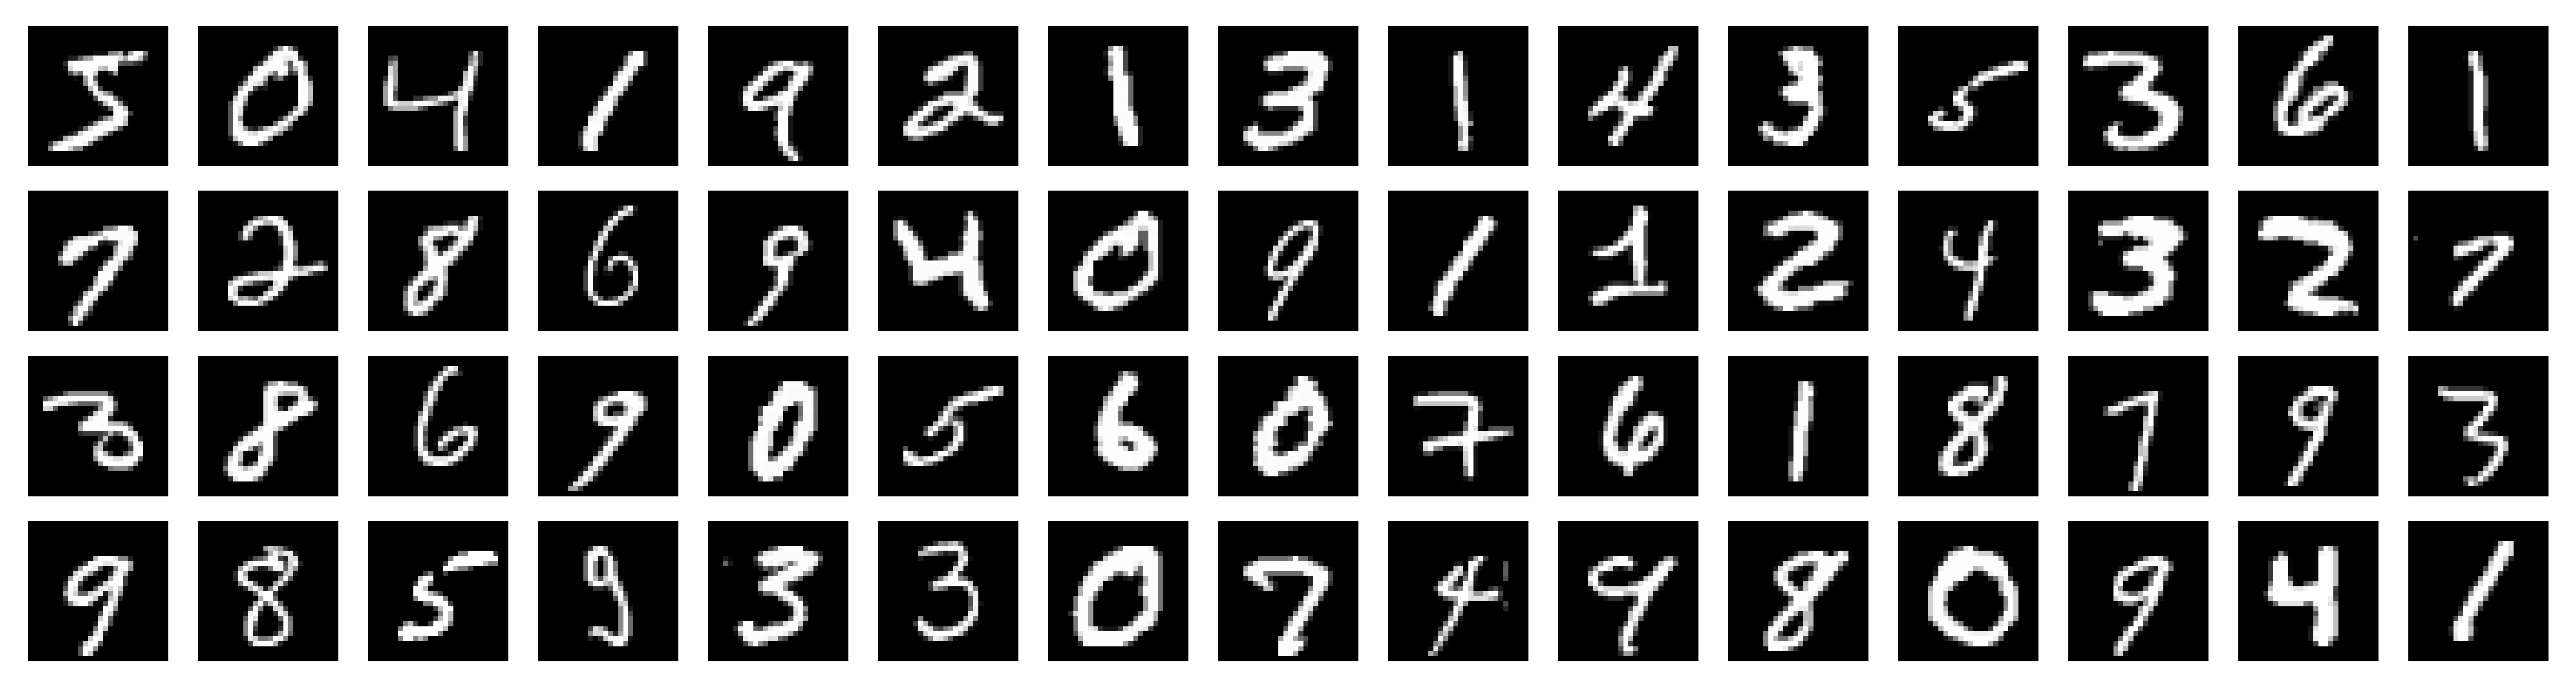
\includegraphics[width=0.9\textwidth]{images/mnist_60_images_4x15_grid.png}
  \caption{Images from the MNIST training set.}
  \label{fig:mnist_images}
\end{figure}

\level{4}{Preprocessing }

\level{3}{Approaches}
\level{4}{Linear Classifier}
\level{4}{Linear Classifier with $L_2$ Norm}
\level{4}{Linear Classifier with $\kappa_2$ Minimization}


